\section{Background and Related Work}
\label{sec:background}

This section defines rules, matches, the multiway evolution graph and the causal and branchial
relations, and reviews related systems.

\subsection{Hypergraph Rewriting Systems}

A \emph{hypergraph} $\hypergraph = (V, E)$ consists of a vertex set $V$ and a set of hyperedges $E$, where each hyperedge $e \in E$ is an ordered tuple of vertices $(v_1, v_2, \ldots, v_k)$ with $v_i \in V$. The Wolfram Physics Project uses hypergraphs because distance in them is path length, which gives rewriting a notion of locality without fixing a space in advance, as strings and cellular automata do.

\begin{definition}[Rewriting Rule]
A rewriting rule $\rewriterule = (L, R)$ consists of a left-hand side pattern $L$ and right-hand side replacement $R$, both hypergraphs. A \emph{match} of $L$ in $\hypergraph$ is an injective mapping $\phi: V_L \to V_\hypergraph$ such that the image of each hyperedge in $L$ appears in $\hypergraph$.
\end{definition}

Rules are applied in the single-pushout form: the matched image is deleted and the replacement glued in, without the gluing conditions of the double-pushout construction~\cite{ehrig2006fundamentals,rozenberg1997handbook,plump2009graph}. Applying rule $\rewriterule$ at match $\phi$ produces a new hypergraph $\hypergraph'$ by:
\begin{enumerate}
    \item Removing all hyperedges in $\phi(L)$ from $\hypergraph$
    \item Adding hyperedges from $R$, extending $\phi$ to map new vertices in $R$ to fresh vertices
\end{enumerate}

\subsection{Multiway Evolution}

\emph{Multiway evolution} applies every applicable rule at every match of every state, producing a directed graph of states connected by events. Figure~\ref{fig:worked-example} shows two steps of a small rule in full: the raw states, the canonical states they reduce to, the events and the causal edges.

\begin{definition}[Evolution Graph]
Given initial state $\state_0$ and rule set $\{\rewriterule_i\}$, the evolution graph $G = (\state, \event)$ contains:
\begin{itemize}
    \item States $\state$: all hypergraphs reachable from $\state_0$
    \item Events $\event$: transitions $(s, s', r, \phi)$ where state $s$ rewrites to $s'$ via rule $r$ at match $\phi$
\end{itemize}
\end{definition}

\begin{figure*}[htbp]
\centering
% GENERATED by tools/dev/object_figure.wls -- do not edit.
% commit 316a7384 | measured on fly_desktop2 | raw states 4, canonical 3, events 3, causal 2, branchial 0 | source: tools/dev/object_figure.wls
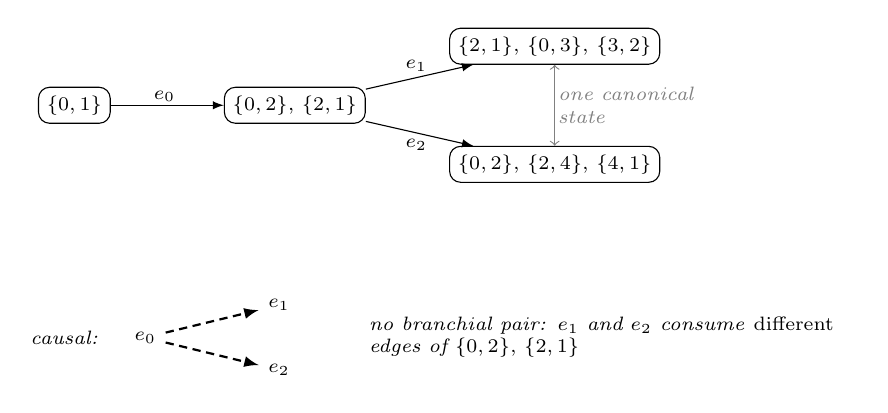
\begin{tikzpicture}[
    st/.style={rectangle, draw, rounded corners, inner sep=3pt, font=\scriptsize},
    ev/.style={->, >=latex, thin},
    cau/.style={->, >=latex, thick, densely dashed},
    lbl/.style={font=\scriptsize\itshape, inner sep=1pt}
]
\node[st] (s0) at (0,0.0) {$\{0,1\}$};
\node[st] (s1) at (2.8,0.0) {$\{0,2\},\,\{2,1\}$};
\node[st] (s2) at (6.1,0.75) {$\{2,1\},\,\{0,3\},\,\{3,2\}$};
\node[st] (s3) at (6.1,-0.75) {$\{0,2\},\,\{2,4\},\,\{4,1\}$};
\draw[ev] (s0) -- node[lbl, above left, pos=0.6]{$e_{0}$} (s1);
\draw[ev] (s1) -- node[lbl, above left, pos=0.6]{$e_{1}$} (s2);
\draw[ev] (s1) -- node[lbl, below left, pos=0.6]{$e_{2}$} (s3);
\draw[<->, gray, thin] (s2) -- node[lbl, right, text width=2.1cm]{one canonical state} (s3);
\node[lbl, anchor=west] at (-0.6,-2.95) {causal:};
\node[font=\scriptsize] (c0) at (0.9,-2.95) {$e_{0}$};
\node[font=\scriptsize] (c1) at (2.6,-2.5375) {$e_{1}$};
\node[font=\scriptsize] (c2) at (2.6,-3.3625) {$e_{2}$};
\draw[cau] (c0) -- (c2);
\draw[cau] (c0) -- (c1);
\node[lbl, anchor=west, text width=6.2cm] at (3.7,-2.95) {no branchial pair: $e_{1}$ and $e_{2}$ consume \emph{different} edges of $\{0,2\},\,\{2,1\}$};
\end{tikzpicture}

\caption{Two steps of $\{x,y\} \rightarrow \{x,z\},\{z,y\}$ from a single edge, as the engine
reports them. Four raw states reduce to three canonical states, because the two depth-2 results
are isomorphic. Both causal edges come from $e_0$, because each depth-2 event consumes one of the
two edges $e_0$ produced. The branchial relation is empty: $e_1$ and $e_2$ start from the same
state but consume different edges. Every element is taken from the engine's output.}
\label{fig:worked-example}
\end{figure*}

The \emph{causal graph} has an edge from event $p$ to event $c$ when $c$ consumes an edge that $p$ produced. The \emph{branchial graph} has an edge between two events that consume a common edge of the same state; it records where the evolution branches, which the Wolfram Physics Project relates to quantum superposition~\cite{wolfram2020project}.

\subsection{The Graph Isomorphism Problem}

Deduplicating states requires deciding whether two hypergraphs are isomorphic, that is, equal up to a relabeling of vertices. Graph isomorphism is in NP and is not known to be NP-complete or to be in P~\cite{kobler2012graph}; the best known algorithm is quasipolynomial~\cite{babai2016quasipolynomial}. This engine computes an exact canonical form for every state, so its canonical hash is equal for two states if and only if they are isomorphic (Section~\ref{sec:canonicalization}).

\subsection{Related Work}

\textbf{Graph canonicalization:} The nauty/Traces line of work~\cite{mckay2014practical} established individualization--refinement (IR) as the standard exact method for graph canonicalization. It is exponential in the worst case and fast on typical instances, and it is the canonicalizer this engine uses. Weisfeiler--Leman color refinement~\cite{weisfeiler1968reduction,shervashidze2011weisfeiler} runs in polynomial time but gives the same value to some non-isomorphic graphs, so it cannot serve as an exact identity.

\textbf{Hypergraph rewriting implementations:} SetReplace~\cite{setreplace} is the implementation
most closely associated with the Wolfram Physics Project, and it computes a different object. Its
multiway construction is a token--event graph over one growing pool of tokens: its vertices are
tokens and events rather than states, a token consumed by one event remains available to others,
and no state identity is computed. Its only isomorphism test during evolution is an optional
deduplication of events with the same input tokens and isomorphic outputs. This engine enumerates
the states graph under exact isomorphism, which requires canonicalizing every state as it is
produced (Section~\ref{sec:canonicalization}), so canonicalization rather than matching dominates
its cost. A wall-time comparison between the two would compare different computations.
Section~\ref{sec:benchmarks} therefore compares against two implementations of the same object: the
\texttt{Wolfram/\allowbreak Multicomputation} paclet's
\texttt{MultiwaySystem}~\citep{wolframmulticomputation}\footnote{Distributed through the Wolfram
Paclet Repository,
\url{https://resources.wolframcloud.com/PacletRepository/resources/Wolfram/Multicomputation/}.
Every comparison uses version 0.1.8, the latest published release (23 November 2024; checked 31
August 2026).}, all of whose properties return Wolfram \texttt{Graph} objects, so its time
includes building them; and this project's \emph{reference implementation}, a direct transcription
of the definition that returns data rather than graphs and serves as the correctness oracle
throughout. \emph{Reference implementation} always means the latter.

\textbf{Subgraph matching on hypergraphs:} HGMatch~\cite{yang2023hgmatch} matches one hyperedge at a time rather than one vertex at a time, seeding a join from one pattern hyperedge and extending it by one hyperedge per step; it restricts candidates by a label-derived signature, and runs as a dataflow on a work-stealing task scheduler. This engine's matcher uses all three. Hyperedges here are unlabelled, so the signature is the edge's vertex-repetition pattern (Definition~\ref{def:signature}). When an expansion has a variable already bound, its candidates come from the vertex index rather than the signature bucket; on the device this reduced match-kernel time on one workload from 944\,ms to 4\,ms.

\textbf{GPU graph algorithms:} GPUs have been applied to subgraph matching~\cite{tran2015fast}, graph mining~\cite{chen2021pangolin} and general graph algorithms~\cite{wang2016gunrock}. This engine's match kernel follows the warp-centric organization of G2Miner~\cite{chen2022g2miner}: one block per (state, rule) pair, its threads dividing the seed candidates and each running its own depth-first search. Unlike these systems, the kernel stays resident across evolution steps, because each step's output states are the next step's inputs.

\textbf{Dynamic graph algorithms:} The causal graph's transitive reduction is maintained as edges are added. Goranci et al.~\cite{goranci2025dynamic} give fully dynamic transitive-reduction algorithms under insertions and deletions in $\BigO(m + n\log n)$ amortized time. This engine's case has insertions only, arriving in topological order, from concurrent workers, and the retained edge set must not depend on the schedule (Section~\ref{sec:tr}).

\textbf{Term rewriting:} Term rewriting theory~\cite{baader1998term} treats confluence and termination for tree-structured terms, and fast implementations~\cite{van2019fastest} optimize similar pattern matching. In hypergraph rewriting the objects are graphs, so matching is subgraph matching rather than tree matching, and states are compared up to isomorphism rather than syntactic equality.

% ----------------------------------------------------------------------------
% CANONICALIZATION
% ----------------------------------------------------------------------------
